\section{Simulation} \label{Sec_Sim}
The simulation was carried out to answer important design questions before the real implementation phase. Furthermore, artificial RFID reader data was created to test and simulate the algorithm, which will be explained in chapter \ref{Sec_Imp}. \\
To answer the design questions, the simulation has the following parameter (Appendix \ref{Sec_AppA} Line 1-50):\begin{itemize}
	\item the size of the simulation space
	\item distance between the tags
	\item distance between the first/last row/column of tags and the boarder of the simulation space
	\item diameter of the robot
	\item position of the antenna related to the origin of the robot
	\item the relation between RSSI and the distance antenna and tag
	\item initial start position and orientation
	\item difference between the measurement points of the initialization procedure
	\item optional: cycle time and speed of the robot (for another procedure)
	\item logging parameter (look of the logged text file)
\end{itemize}	
Foregone tests lead to a distance between the tags of 10 cm. This was founded on the fact that in this case at least four tags are detected at the same time (maximum reading range of 14 cm). In this case around 121 tags are needed for every square meter. This is a realistic number of tags for a small plant size, because it will lead to around 800 tags for the whole plant. \\

\subsection{Emulator}
To create artificial RFID reader data, the emulator must write all detected tags together with information about the measuring point into a text file. During the initialization procedure, which was the main focus in this project, the robot turns around 360 $^\circ$ and makes measurements every 45$^\circ$. \\
The emulator computes the distance from the center of the antenna to the neighbouring tags at each measurement point. If a tag is closer than the maximal reading distance, the emulator writes the detected ID of the tag together with its RSSI into the text file. \\
The RSSI is, as explained earlier, an integer value from 0...7. 0 defines in this case a distance from 14 to around 10 cm from the antenna to the tag. In the first version of the emulator the RSSI mentioned a consistent increasing of the RSSI while the distance between the tags and the antenna gets smaller \cite{ChristofRohrigDanielHessandFrankKunemund.}. \\
During own measurements it has been found out that this relation is inconsistent. Therefore the second version of the emulator was updated and creates more realistic data.\\

\subsection{RSSI Measurements with real hardware}\label{Sec_Sim_Mea}
The relation of the RSSI is not just related to the distance between the antenna and the tag. It also depends on the orientation of the plain of the antenna and the tag. The tests with the real hardware was performed in a setup where the tags were placed on a floor and the antenna was parallel to the floor at a hight of 1.5 cm. The reason for this was the fact that the antenna should be placed directly under the robot. Table. \ref{RSSI_Dis_data} and fig. \ref{RSSI_Dis} present the results of the measurements.\\
\begin{table}[!htbp]
\centering
\begin{tabular}{|c|c|c|c|c|c|c|c|c|}
\hline
\begin{tabular}[c]{@{}c@{}}RSSI \\ (Received Signal Strength Indicator) \end{tabular}  & 0/0 & 1/1 & 2/2 & 3/3 & 4/4 & 5/5 & 6/6 & 7/7 \\ \hline
\begin{tabular}[c]{@{}c@{}}Maximal distance \\ antenna to tag [cm]\end{tabular} & 14  & 9.8 & 9   & 8   & 7   & 6   & 3.5 & 2.8 \\ \hline
\begin{tabular}[c]{@{}c@{}}Middle distance\\ antenna to tag [cm]\end{tabular}   & 5   & 5.1 & 5.3 & 5.5 & 5.8 & 4   & -   & -   \\ \hline
\begin{tabular}[c]{@{}c@{}}Minimal distance\\ antenna to tag [cm]\end{tabular}  & -   & 4.7 & 4.5 & 4.3 & 4.2 & -   & -   & -   \\ \hline
\end{tabular}
\caption{Relation between RSSI and distance antenna to tag (data)}
\label{RSSI_Dis_data}
\end{table}\\
\begin{figure}[!htbp]
\centering
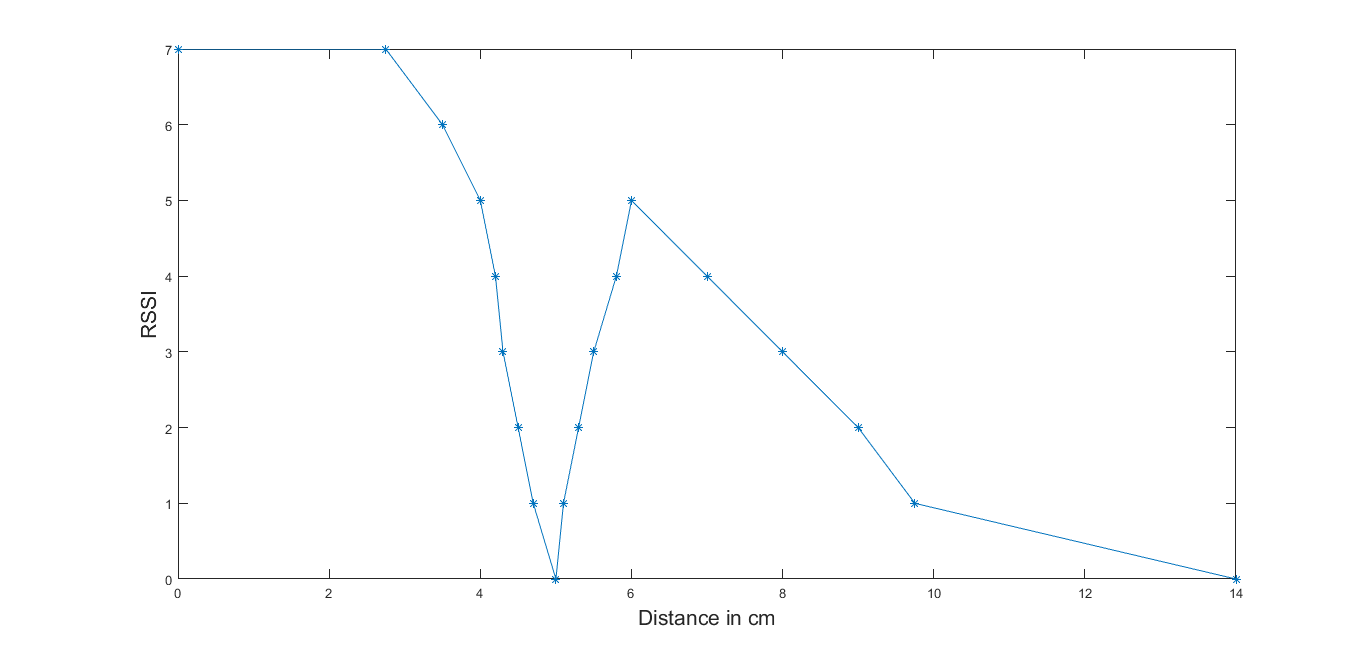
\includegraphics[width = 14cm]{Pictures/RSSI_Distance}
\caption{Relation between RSSI and distance antenna to tag}
\label{RSSI_Dis}
\end{figure}\\
Figure \ref{RSSI_Dis} demonstrates that there exists a blind spot at a distance of 5 cm where the RSSI drops to 0. The consequence is that it is not trivial to build up a relation from the RSSI back to the correct distance. \\

\subsection{Simulation with emulated data}
The idea of the final implementation is to estimate the initial position and orientation of the robot. A first version of an algorithm to solve this problem is created in matlab. The first part of these algorithm is the emulator which simulates the 360$^\circ$ turn and records the tag information. The second part is the solver which is also explained in depth in the section \ref{Sec_Imp}. \\
After observing an inconsistent behaviour of the RSSI the simulation as well as the solver were updated.\\

\subsection{Results}
The application of the emulated data on the solver indicates the following results: \\
\begin{table}[!htbp]
\centering
\begin{tabular}{|c|c|c|}
\hline
                               & \begin{tabular}[c]{@{}c@{}}Avg. accuracy position \\  (x-, \& y-direction) {[}mm{]}\end{tabular} & \begin{tabular}[c]{@{}c@{}}Avg. Accuracy \\  orientation [$^\circ$] \end{tabular} \\ \hline
Data mentioned in paper        & 2                                                                                                  & \textless{}1                                                                    \\ \hline
Own recorded data (blind spot) & 10                                                                                                 & 20                                                                              \\ \hline
\end{tabular}
\caption{Results Simulation}
\label{Res_Sim}
\end{table}\\
As can be seen from table. \ref{Res_Sim}, there is a sufficient good match between the estimated position and orientation of the robot for the consistent RSSI data. On the other hand the inconsistent RSSI data results in significant differences in the estimation of the position and orientation of the robot.\\
The reason for this is the higher complexity of the algorithm to first estimate the correct distances related to RSSI values and then start to estimate the position based on those distances. \\
A small error in the estimation of the position of the antenna at the first measurement point leads also to a big error in the computed orientation of the robot.

 